% ch/ht3.tex: Sections 10 to 12 of the chapter of N. Polson (curved boundaries, Yor's function, the Davenport Heilbronn test), editor E2. Labels ht:*. Status words: proved, computed, conditional, heuristic, open. Numbers are those of misc/reviews/nick-hitting_times/checks-G2.md. Labels of ht1, ht2 and ht5 used here: ht:thm:32, ht:thm:rigid, ht:cor:shape, ht:sec:families, ht:prob:rs, ht:prob:yor.
\section{Curved boundaries: the Roberts and Shortland view}\label{ht:sec:rs}

Roberts and Shortland \cite{RS95} compute the law of the first time a Brownian motion crosses a curved, time dependent boundary, the problem behind barrier options with time dependent coefficients. Their question runs from boundary to law. Ours runs the other way: for a law $\nu$ on $(0,\infty)$, find $b$ such that
\[
\tau_b=\inf\{t>0: W_t\ge b(t)\},\qquad W_0=0,
\]
has law $\nu$. This is the inverse first passage problem. Under mild conditions on $\nu$ it has a unique solution, in a suitable viscosity sense \cite{Anulova80,CCCS11}. So $\mu$ has a boundary whether or not RH holds, and the existence of the representation says nothing. The question is whether the boundary has a shape that sees the zeros. The boundary of $\mu$ is the one computed in Section~\ref{ch:boundaries} and in Sections~\ref{ch:bphit} and \ref{ch:bpeta}; here we add the enclosure at small times, the validation of the solver, and the effect of moving a zero. Three statements result: the two ends of the boundary are determined by quantities that do not depend on RH (Proposition~\ref{ht:prop:smallb} and the slope at infinity); the boundary in between is computed to about $2\cdot10^{-4}$; and moving a zero off the line changes it, to first order and heuristically, by an amount proportional to $\delta^2/\gamma^4$ times a profile that does not depend on the zero (Remark~\ref{ht:rem:resp}).

\subsection{The small time end}

\begin{proposition}\label{ht:prop:smallb}
Let $b$ be the boundary of $\mu$, write $F(t)=\mu(0,t]$, and let $m(t)=\inf_{0<s\le t}b(s)$. For every $t>0$,
\[
\sqrt t\,\bar\Phi_{\mathrm N}^{-1}\big(F(t)\big)\le b(t),\qquad m(t)\le\sqrt t\,\bar\Phi_{\mathrm N}^{-1}\big(\tfrac12F(t)\big),
\]
where $\Phi_{\mathrm N}$ is the standard normal distribution function and $\bar\Phi_{\mathrm N}=1-\Phi_{\mathrm N}$. Moreover $-\log F(t)\sim(\log(1/t))^2/(16t)$ as $t\downarrow0$, so
\[
\liminf_{t\downarrow0}\frac{b(t)}{\log(1/t)}\ge\frac1{2\sqrt2},\qquad \limsup_{t\downarrow0}\frac{m(t)}{\log(1/t)}\le\frac1{2\sqrt2},
\]
and if $b$ is nonincreasing near $0$ then $b(t)\sim\log(1/t)/(2\sqrt2)$. None of this depends on RH. Status: proved.
\end{proposition}

\begin{proof}
If $W_t\ge b(t)$ then $\tau_b\le t$, so $\bar\Phi_{\mathrm N}(b(t)/\sqrt t)\le F(t)$, which is the first inequality. If $\tau_b\le t$ then $\sup_{s\le t}W_s\ge m(t)$, and by the reflection principle $F(t)\le2\bar\Phi_{\mathrm N}(m(t)/\sqrt t)$, which is the second. For the asymptotics, Stirling's formula and $\zeta(\sigma)\to1$ give $-\log\E e^{-s\tau}=\log\xi(\frac12+\sqrt s)-\log\xi(\frac12)\sim\frac14\sqrt s\log s$ as $s\to\infty$ through the reals, unconditionally. This is regularly varying of index $\frac12$, and Kasahara's exponential Tauberian theorem \cite{Kasahara78}, \cite[Section 4.12]{BGT87} % UNCHECKED: section number of BGT87 not verified
converts it into the Legendre transform asymptotics: the supremum of $\frac14\sqrt s\log s-st$ is attained at $\sqrt s\sim\log(1/t)/(4t)$ and equals $(\log(1/t))^2/(16t)$ to leading order. Since $\bar\Phi_{\mathrm N}^{-1}(p)\sim\sqrt{2\log(1/p)}$ as $p\downarrow0$, both bounds become $\sqrt{2t\cdot(\log(1/t))^2/(16t)}=\log(1/t)/(2\sqrt2)$. When $b$ is nonincreasing, $m=b$ and the two bounds meet.
\end{proof}

The proposition is also a check on the numerics. For a nonincreasing boundary the two bounds enclose $b$, and they are explicit in $F$. Evaluating the Legendre transform numerically (computed), the ratio $b(t)/\log(1/t)$ is $0.269$, $0.328$, $0.342$, $0.348$ at $t=10^{-4},10^{-8},10^{-12},10^{-16}$, approaching $1/(2\sqrt2)=0.354$ slowly, as the $\log\log$ corrections suggest. Every finite sum of exponentials has a polynomial lower tail and hence $b(0+)=0$. The logarithmic blow up is the trace of infinitely many zeros, through the growth of $\xi$ along the real axis, and it is the same wherever the zeros lie.

\subsection{Computing the boundary}
Conditioning on the crossing time and using the strong Markov property gives, for every $t>0$,
\[
\bar\Phi_{\mathrm N}\Big(\frac{b(t)}{\sqrt t}\Big)=\int_0^t\bar\Phi_{\mathrm N}\Big(\frac{b(t)-b(s)}{\sqrt{t-s}}\Big)\,\nu(\mathrm ds),
\]
a nonlinear Volterra equation of the first kind for $b$ \cite{Peskir02}. We solve it forward with a midpoint rule in $s$. At each step the right side minus the left side need not be monotone in $b(t)$, and a global root search occasionally jumps to a spurious root; bracketing the root next to the previous value removes this. The distribution function of $\mu$ comes from a contour integral of $\xi(\frac12)/(s\,\xi(\frac12+\sqrt s))$ along a vertical line through the saddle point below $t=0.0064$ and from the residue expansion with $120$ zeros above it; the two agree to a relative difference of $10^{-33}$ where they overlap. The code is \texttt{code/ht\_curved.py}. We validated the solver in three ways (all computed).
\begin{enumerate}
\item On the linear boundary $b(t)=1-t/2$, whose crossing law is known in closed form, it recovers $b$ to $10^{-6}$ for $t\ge0.05$; the start of the recursion carries a transient of a few $10^{-3}$ that does not reach the range of interest.
\item Halving the step from $4\cdot10^{-5}$ to $2\cdot10^{-5}$ changes the boundary of $\mu$ by at most $1.5\cdot10^{-4}$ on $[0.0045,0.12]$, at most $8\cdot10^{-5}$ for $t\ge0.006$, and at most $2.2\cdot10^{-5}$ for $t\ge0.01$.
\item The computed boundary is decreasing, and at every grid point it lies inside the enclosure of Proposition~\ref{ht:prop:smallb}, whose width is $0.004$ at $t=0.0045$ and $0.015$ at $t=0.01$. Figure~\ref{ht:fig:ifpt}(b) compares the boundary at small times with the asymptote $\log(1/t)/(2\sqrt2)$ of Proposition~\ref{ht:prop:smallb}.
\end{enumerate}
The interval $[0.0045,0.12]$ carries all but about $2\cdot10^{-9}$ of the mass of $\mu$, whose mean is $0.0231$.

\subsection{The large time end and the shape}
The tail $\mu(t,\infty)\sim c\,e^{-\gamma_1^2t}$ forces $b'(t)\to-\sqrt2\,\gamma_1=-19.99$, the slope of a Brownian motion whose drift gives hitting hazard $\gamma_1^2$. Matching the survival function of a Brownian motion with drift $c=\sqrt2\,\gamma_1$ below a slowly rising level $g(t)$, namely $\mathrm{const}\cdot g\,t^{-3/2}e^{cg-c^2t/2}$, against $c'e^{-\gamma_1^2t}$ gives $cg+\log g=\frac32\log t+O(1)$, so (heuristic: the matching is quasi static and has no error control)
\begin{gather*}
b(t)=-\sqrt2\,\gamma_1t+\frac{3}{2\sqrt2\,\gamma_1}\log t-\frac{1}{\sqrt2\,\gamma_1}\log\log(\gamma_1^2t)+O(1),\\
t\big(b'(t)+c\big)\to\frac3{2c}.
\end{gather*}
We checked this in two ways (computed). For the exponential law, $t(b'+\sqrt2)$ is $0.80$, $0.88$, $0.92$, $0.94$ at $t=20,50,100,150$, against $3/(2\sqrt2)-1/(\sqrt2\log t)=0.82$, $0.88$, $0.91$, $0.92$. For $\mu$ we continued the solution to $t=2$ with the complementary form of the integral equation, $\Phi_{\mathrm N}(b(t)/\sqrt t)-\mu(t,\infty)=\int_0^t\Phi_{\mathrm N}((b(t)-b(s))/\sqrt{t-s})\,\mu(\mathrm ds)$, which keeps full relative accuracy when the survival function is as small as $e^{-400}$. Then $t(b'+c)$ is $0.0645$, $0.0665$, $0.0677$, $0.0688$ at $t=0.8,1.2,1.6,2$, against $0.0652$, $0.0659$, $0.0664$, $0.0667$ from the formula, with $3/(2c)=0.0750$ as the limit. The limit is not reached on the range computed, and the slow approach seen on $[0.03,0.12]$, where the slope is still $-19.6$ at the right end, is consistent with the $\log t$ correction rather than with a numerical artefact. This end sees only the first zero, which is on the line.

Between the two ends the shape gives no criterion either. The exponential law, the simplest GGC, has a boundary that starts at $0$, rises to a maximum of $0.664$ at $t=0.25$, and then falls with slope tending to $-\sqrt2$; the Gamma law of shape $2$ behaves the same way. The boundary of $\mu$ falls monotonically from $+\infty$. GGC boundaries thus come in shapes that no simple convexity or monotonicity condition separates.

\subsection{Moving a zero off the line}
To see what a zero off the line does, we replace one factor $1+s/\gamma_m^2$ of the Hadamard product by the pair $(1+s/\lambda)(1+s/\bar\lambda)$ with $-\lambda=(\delta+i\gamma_m)^2$, the image of the quartet $\frac12\pm\delta\pm i\gamma_m$. As a GGC control we use the split real pair $(\gamma_m\pm0.001)^2$, so that both laws have the same number of factors. The value $\delta=0.3085$ is the displacement of the Davenport Heilbronn zero of Section~\ref{ht:sec:dh}.

\begin{table}[ht]
\centering\footnotesize
\begin{tabular}{ccccc}
\toprule
zero & $\delta$ & $\max|b_{\mathrm{toy}}-b_{\mathrm{GGC}}|$ & density negative from & a law \\
\midrule
$\gamma_1$ & $0.05$ & $2.25\cdot10^{-4}$ & $t=2.25$ & no \\
$\gamma_1$ & $0.15$ & $2.0\cdot10^{-3}$ & $t=0.77$ & no \\
$\gamma_1$ & $0.3085$ & $8.8\cdot10^{-3}$ & $t=0.39$ & no \\
$\gamma_6$ & $0.3085$ & $8.2\cdot10^{-6}$ & never & yes \\
$\gamma_{20}$ & $0.3085$ & $6.3\cdot10^{-7}$ & never & yes \\
$\gamma_{60}$ & $0.3085$ & $5.5\cdot10^{-8}$ & never & yes \\
\bottomrule
\end{tabular}
\caption{Boundaries with one off line pair against a GGC control on $[0.0045,0.12]$; for $\gamma_{60}$ the maximum is over $[0.0045,0.1]$, since near $t=0.12$ the solver noise of about $2\cdot10^{-7}$ exceeds the signal. ``Never'' means the density was found positive on a grid of step $0.005$ on $(0.0064,6]$ and at three points below $0.0064$, beyond which the tail is governed by $\gamma_1$. All entries computed (\texttt{code/ht\_curved.py}).}\label{ht:tab:ifpt}
\end{table}

When the off line pair is the lowest zero, the pole closest to the origin is complex, the density oscillates in its tail and becomes negative; at $\delta=0.3085$ this happens at $t=0.39$, where the remaining mass is about $e^{-78}$. Beyond that point no boundary exists, and before it the boundary moves by less than $10^{-2}$. For $\xi$ this case cannot occur, because the lowest zero is on the line. When the pair sits higher the tail is still governed by $\gamma_1$, and the toy law is, on the evidence of the computed density, a probability law that is not a GGC (it has complex poles, Theorem~\ref{ht:thm:rigid}). The size of the change then follows a simple rule. Two parts of it are proved.

\begin{proposition}\label{ht:prop:resp}
Moving the pair at height $\gamma$ off the line by $\delta$ multiplies the Laplace transform, relative to the control, by $1+6\delta^2s/\gamma^4+O(\delta^2s^2/\gamma^6)$ for $|s|\ll\gamma^2$. To first order this is the shift $\tau\mapsto\tau-6\delta^2/\gamma^4$ of the mean. Status: proved.
\end{proposition}

\begin{proof}
The mean of a GGC with atoms $\lambda_j$ is $\sum1/\lambda_j$. For the toy pair this contribution is $2\Re(1/\lambda)=2(\gamma^2-\delta^2)/(\gamma^2+\delta^2)^2=2/\gamma^2-6\delta^2/\gamma^4+O(\delta^4/\gamma^6)$, and for the control it is $2/\gamma^2+O(10^{-6}/\gamma^4)$. Higher cumulants change by $O(\delta^2/\gamma^{2k+2})$, and the ratio of the two Laplace transforms is $\big((1+s/\lambda)(1+s/\bar\lambda)\big)^{-1}$ over the control factor, which expands as stated.
\end{proof}

The step from the law to the boundary is not proved, and we state it as an observation.

\begin{remark}[Boundary response, heuristic]\label{ht:rem:resp}
If the map from a law to its boundary is linear to first order and the change of the law is, to leading order, a pure shift, then
\[
b_{\mathrm{toy}}(t)-b_{\mathrm{GGC}}(t)\approx\frac{6\delta^2}{\gamma^4}\,K(t),
\]
where $K$ is the linear response of the boundary to a shift of the law, a profile that does not depend on $\gamma$ or $\delta$. Linearity, the universality of $K$ and the size of the neglected terms are assumed, not proved. Status: heuristic, checked numerically (Table~\ref{ht:tab:resp}).
\end{remark}

We computed $K$ directly by solving for the law of $\tau-\Delta$ with $\Delta=2\cdot10^{-6}$; it is $-72$, $-29$, $-13$, $-11$ at $t=0.01,0.02,0.05,0.08$, and it is linear in $\Delta$ to four digits (the values at $\Delta=2\cdot10^{-6}$ and $4\cdot10^{-6}$ agree to $10^{-2}$). Table~\ref{ht:tab:resp} compares it with the normalised differences $(b_{\mathrm{toy}}-b_{\mathrm{GGC}})\gamma^4/6\delta^2$, and Figure~\ref{ht:fig:ifpt}(c) shows the collapse. At $t=0.02$ the three heights agree with $K$ to $3\%$, $2\%$ and $0.5\%$. At small times the agreement sets in only once $t$ exceeds a multiple of $1/\gamma$, where the relevant $s$ are below $\gamma^2$.

\begin{table}[ht]
\centering\footnotesize
\begin{tabular}{ccccc}
\toprule
& $t=0.01$ & $t=0.02$ & $t=0.05$ & $t=0.08$ \\
\midrule
$\gamma_6$ & $-11.2$ & $-28.3$ & $-17.0$ & $-14.4$ \\
$\gamma_{20}$ & $-36.5$ & $-29.8$ & $-13.7$ & $-11.7$ \\
$\gamma_{60}$ & $-60.6$ & $-29.5$ & $-13.1$ & $-11.2$ \\
$K(t)$ & $-71.9$ & $-29.3$ & $-12.9$ & $-11.0$ \\
\bottomrule
\end{tabular}
\caption{Normalised boundary change $(b_{\mathrm{toy}}-b_{\mathrm{GGC}})\gamma^4/6\delta^2$ against the shift response $K(t)$, $\delta=0.3085$ (computed).}\label{ht:tab:resp}
\end{table}

\begin{figure}[ht]
\centering
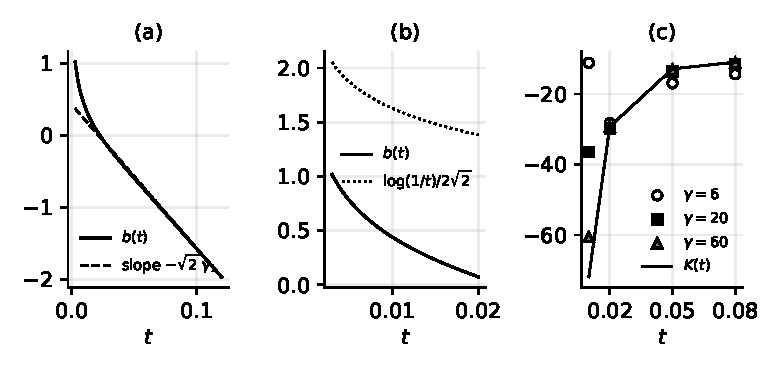
\includegraphics[width=\textwidth]{fig/ht_ifpt.pdf}
\caption{(a) The inverse first passage boundary $b$ of the reciprocal Xi law on $[0.003,0.12]$, with the line of slope $-\sqrt2\,\gamma_1$ through its last node. (b) The boundary at small times against the asymptote $\log(1/t)/(2\sqrt2)$ of Proposition~\ref{ht:prop:smallb}, which it approaches only slowly. (c) Normalised boundary changes for off line pairs at the zeros $6$, $20$, $60$, against the shift response $K$ (computed).}\label{ht:fig:ifpt}
\end{figure}

For $\xi$ the consequence is quantitative, and it is first order and heuristic (Remark~\ref{ht:rem:resp}). Any zero off the line lies above height $3\cdot10^{12}$ \cite{PT21} and has $\delta<\frac12$, so its shift is at most $6\cdot\frac14/(3\cdot10^{12})^4<2\cdot10^{-50}$. The computed response satisfies $|K|\le215$ on $[0.0045,0.12]$ (its computed maximum is $195.5$ at $t=0.0045$). For one off line quartet the boundary of $\mu$ on the range carrying all but $2\cdot10^{-9}$ of the mass would therefore change, to first order, by less than $10^{-47}$. RH failing allows every zero above $3\cdot10^{12}$ to be off the line, and then the first order shifts add up to $\tfrac32\sum_{\gamma>T}\gamma^{-4}\approx8\cdot10^{-38}$ at most, so the change is less than $10^{-34}$ (the computed value of the product with $215$ is $1.7\cdot10^{-35}$; here $\sum_{\gamma>T}\gamma^{-4}\ll T^{-3}\log T$). The change is larger only at times of order $\log\gamma/\gamma$, where the saddle point $s$ reaches $\gamma^2$; by Proposition~\ref{ht:prop:smallb} the mass there is about $\exp(-\frac14\gamma\log\gamma)$.

\subsection{Assessment}
The Roberts and Shortland view is a faithful and cheap encoding of $\mu$: the boundary is computable to about $2\cdot10^{-4}$ on the range that carries the mass, and Proposition~\ref{ht:prop:smallb} gives an explicit enclosure at small times. But its two ends are fixed by the growth of $\xi$ and by the first zero, and a violation of RH would move it in between, to first order (heuristic, Remark~\ref{ht:rem:resp}), by about $6\delta^2\gamma^{-4}K(t)$, which is the same first order shift that any other representation of $\mu$ would show. A shape test could see RH only if it detected the GGC property itself, through a characterisation of the boundaries whose crossing laws are GGCs. Kent's theorem \cite{Kent80} makes the hitting times of levels by one dimensional diffusions GGCs, but we do not know which curved boundaries for Brownian motion reduce to that case, and we record the question as Problem~\ref{ht:prob:rs}. Without such a theorem the method is a computational tool, useful for the prime side laws of Theorem~\ref{ht:thm:32} and the Davenport Heilbronn comparison, with no positivity of its own.

\section{Marc Yor's probabilistic Riemann function}\label{ht:sec:yor}

Marc Yor and his coauthors built a substantial probabilistic account of $\xi$. Four of their papers bear on this chapter: Biane, Pitman and Yor on Brownian laws whose Mellin transform is $\xi$ \cite{BPY01}; Pitman and Yor on the hyperbolic laws \cite{PitmanYor03}; James, Roynette and Yor on GGCs, Thorin measures and Dirichlet means \cite{JRY}; and Nikeghbali and Yor on the Barnes $G$ function \cite{NY09}. We take them in turn and ask of each what it adds to the reciprocal Xi law $\mu$. Section~\ref{ch:biane} and \eqref{bp:eq:bpy} of the basepoint chapter already use the first of these papers; this section adds the harmonic mean form, the Davenport Heilbronn counterpart and the Wiener and Gamma coupling.

\subsection{The Biane, Pitman and Yor variable}
Let $b$ be a standard Brownian bridge and $Y=\sqrt{2/\pi}\,(\max_ub_u-\min_ub_u)$. Biane, Pitman and Yor prove \cite[(4), (5)]{BPY01} % UNCHECKED: equation numbers of BPY01 not verified
\[
\E\,Y^s=2\xi(s)\qquad(s\in\mathbb C).
\]
The same law appears in several Brownian guises: $Y^2\overset{d}{=}\frac\pi2\Sigma_2$ with $\Sigma_2=\frac2{\pi^2}\sum_{n\ge1}(\varepsilon_n+\hat\varepsilon_n)/n^2$, whose Laplace transform is $(\sqrt{2\lambda}/\sinh\sqrt{2\lambda})^2$; $\Sigma_2$ is the sum of two independent hitting times of $1$ by a three dimensional Bessel process; and $\frac\pi2\sqrt{\Sigma_2}$ is the maximum of a standard Brownian excursion \cite[(57)]{BPY01}. % UNCHECKED: equation number (57)
The functional equation $\xi(s)=\xi(1-s)$ becomes the size bias identity $\E g(1/Y)=\E\,Y g(Y)$ \cite[(20)]{BPY01}. % UNCHECKED: equation number (20)
The reciprocal of $\xi$ follows at once.

\begin{proposition}\label{ht:prop:bpy}
Let $\mathbb P^*$ have density $Y^{1/2}/\E Y^{1/2}$ with respect to $\mathbb P$, and let $U=\log Y$. Under $\mathbb P^*$ the variable $U$ is symmetric and has the law of the P\'olya variable of \eqref{eq:ch2:mgf}, with density $\Phi/\Xi(0)$, where $\Xi(z)=\xi(\frac12+iz)$ and $\Phi$ is the kernel of Riemann and P\'olya of \eqref{eq:ch2:Phi}; equivalently $U/2$ has density $2\Phi(2u)/\Xi(0)$. Moreover
\[
\E\,e^{-s\tau}=\frac{\xi(\frac12)}{\xi(\frac12+\sqrt s)}=\frac1{\E^*\cosh(\sqrt s\,U)}=\frac1{\E^*\big[\E[e^{-sT}\,|\,U]^{-1}\big]},
\]
where, given $U$, $T$ is the exit time of a standard Brownian motion from $(-|U|/\sqrt2,|U|/\sqrt2)$. Status: proved.
\end{proposition}

\begin{proof}
From $\E Y^s=2\xi(s)$, $\E^*e^{wU}=\E\,Y^{1/2+w}/\E\,Y^{1/2}=\xi(\frac12+w)/\xi(\frac12)$. Taking $g(y)=y^{-1/2}f(\log y)$ in the size bias identity gives $\E\,Y^{1/2}f(-\log Y)=\E\,Y^{1/2}f(\log Y)$, so $U$ is symmetric under $\mathbb P^*$ and $\E^*e^{wU}=\E^*\cosh(wU)$. Putting $w=iz$ gives $\E^*e^{izU}=\Xi(z)/\Xi(0)=\int_{\mathbb R}\Phi(u)e^{izu}\mathrm du/\Xi(0)$, which identifies the density of $U$ (this is \eqref{eq:ch2:mgf}). Finally $\E e^{-sT}=1/\cosh(a\sqrt{2s})$ for exit from $(-a,a)$, and $a=|U|/\sqrt2$.
\end{proof}

So the harmonic mean route of Section~\ref{ht:sec:families} has an explicit Brownian mixing variable: the logarithm of the normalised range of a Brownian bridge, size biased by its square root. Each conditional exit time is a GGC, and $\mu$ is a GGC exactly when the harmonic mean over $U$ preserves that property, which is RH. Proposition~\ref{ht:prop:bpy} puts the problem in Brownian language without changing it.

\subsection{Davenport and Heilbronn have the same structure}
The Biane, Pitman and Yor structure rests on two facts: the theta function behind $\xi$ is positive, and it is self dual. The Davenport Heilbronn function shares both.

\begin{proposition}\label{ht:prop:dhtheta}
Let $a_n$ be the Davenport Heilbronn coefficients, periodic modulo $5$ with $(a_0,\dots,a_4)=(0,1,\kappa,-\kappa,-1)$ and $\kappa=0.2840790438$, and let $\theta_{DH}(x)=\sum_{n\ge1}a_nn\,e^{-\pi n^2x/5}$. Then $\theta_{DH}(x)>0$ for every $x>0$. Consequently there is a probability law on $(0,\infty)$ whose Mellin transform is a constant multiple of $\xi_{DH}$, a symmetric $U_{DH}$ with $\E^*e^{wU_{DH}}=\xi_{DH}(\frac12+w)/\xi_{DH}(\frac12)$, and a positive P\'olya kernel $\Phi_{DH}$. Status: proved.
\end{proposition}

\begin{proof}
For $x\ge1$, using $|a_n|\le1$,
\[
\theta_{DH}(x)\ge e^{-\pi x/5}\Big(1-\sum_{n\ge2}n\,e^{-\pi(n^2-1)x/5}\Big)\ge e^{-\pi x/5}(1-0.324)>0 .
\]
The functional equation of $f_{DH}$ is equivalent to the self duality $\theta_{DH}(1/x)=x^{3/2}\theta_{DH}(x)$, which we also checked numerically (to a relative $10^{-40}$ at $37$ points), and it carries positivity to $0<x<1$. Mellin transformation gives $\int_0^\infty\theta_{DH}(x)x^{(s+1)/2}\,\mathrm dx/x=\sqrt{5/\pi}\,\xi_{DH}(s)$ (checked to $2\cdot10^{-41}$ at $s=\frac12$ and $s=0.8+i$), so $\theta_{DH}(x)x^{1/2}/x$, normalised, is a probability density with Mellin transform $\xi_{DH}(s)/\xi_{DH}(0)$ in the variable $s/2$. The rest follows as in Proposition~\ref{ht:prop:bpy}.
\end{proof}

The harmonic mean $1/\E^*\cosh(\sqrt s\,U_{DH})$ has the complex pole $s=(0.3085+85.699i)^2$ coming from the off line zero, so it is not a GGC (Theorem~\ref{ht:thm:rigid}). The positivity of a self dual kernel, the size bias symmetry and the harmonic mean representation therefore all hold for a function that violates RH. What Davenport and Heilbronn may lack is the Brownian meaning: we do not know whether $\theta_{DH}$ is the theta function of any natural Brownian or Bessel functional. That is the only place in the Biane, Pitman and Yor picture where arithmetic could enter, and we record it as Problem~\ref{ht:prob:yor}.

\subsection{The hyperbolic laws as solvable models}
Pitman and Yor \cite{PitmanYor03} study the laws $C_1$, $S_1$, $T_1$ with Laplace transforms $1/\cosh\sqrt{2s}$, $\sqrt{2s}/\sinh\sqrt{2s}$ and $\tanh\sqrt{2s}/\sqrt{2s}$. The first is the exit time of Brownian motion from $(-1,1)$, and
\[
\frac1{\cosh\sqrt{2s}}=\prod_{n\ge1}\Big(1+\frac{2s}{\pi^2(n-\frac12)^2}\Big)^{-1}
\]
is the exact model of $\mu$ under RH, with $\pi^2(n-\frac12)^2/2$ in place of $\gamma_n^2$: a GGC whose Thorin measure is a sum of unit atoms, of infinite total mass \cite[Section 1.6]{JRY}. % UNCHECKED: section number of JRY not verified
The law $T_1$ shows how a GGC fails. Its transform has zeros and poles interlacing on the negative axis, so its Thorin measure has atoms of both signs, and it is not a GGC \cite{JRY}. For $\mu$ an off line zero produces instead a pair of complex atoms. Both failures are visible only in the canonical function, not in positivity of the law.

\subsection{The Wiener and Gamma representation}
James, Roynette and Yor \cite[Proposition 1.1]{JRY} % UNCHECKED: proposition number of JRY not verified
show that a positive variable is a GGC if and only if it is a Wiener and Gamma integral $\int_0^\infty h(u)\,\mathrm d\gamma_u$ against a standard gamma process, where the Thorin measure is the image of Lebesgue measure under $u\mapsto1/h(u)$, and $h$ can be taken nonincreasing and is then unique. For $\mu$ under RH this gives $h(u)=1/\gamma_{\lceil u\rceil}^2$ and $\mu=\sum\varepsilon_n/\gamma_n^2$.

The base point laws $\mu^{(\alpha)}$ with transform $\xi(\alpha)/\xi(\alpha+\sqrt s)$ fit the same frame, but only when $\alpha\ge\sup_\rho\Re\rho$, which is where $\mu^{(\alpha)}$ is a GGC (Theorem~\ref{thm:poisson}; below that line the Hadamard product has zeros in the slit plane and no Thorin representation exists, see Proposition~\ref{ag:prop:factor}). For such $\alpha$ the Hadamard product gives
\begin{gather*}
\log\frac{\xi(\alpha+\sqrt s)}{\xi(\alpha)}=\int_0^\infty\log\Big(1+\frac s{t^2}\Big)\,\mathrm dN_\alpha(t),\\
N_\alpha'(t)=\frac1\pi\Re\frac{\xi'}{\xi}(\alpha+it)=\frac1\pi\sum_\rho\frac{\alpha-\beta}{(\alpha-\beta)^2+(t-\gamma)^2},
\end{gather*}
so the Thorin measure in the variable $t$ is $\mathrm dN_\alpha$, a Poisson smoothing of the zero counting function at width $\alpha-\beta$. Then $\mu^{(\alpha)}$ is the Wiener and Gamma integral of $h_\alpha(u)=N_\alpha^{-1}(u)^{-2}$. The density $N_\alpha'$ is also defined for $\alpha<\sup_\rho\Re\rho$, and its positivity on every line $\Re s=\alpha>\frac12$ is Lagarias's criterion (Remark~\ref{rem:ch2:oneline}), but on a single such line positivity of the density does not make $\mu^{(\alpha)}$ a GGC.

\begin{proposition}\label{ht:prop:wg}
On one gamma process $\gamma$, set $X_\alpha=\int_0^\infty h_\alpha(u)\,\mathrm d\gamma_u$. Then $X_\alpha$ has law $\mu^{(\alpha)}$ for every $\alpha\ge\sup_\rho\Re\rho$, in particular for every $\alpha\ge1$. RH holds if and only if $N_\alpha$ is nondecreasing for every $\alpha>\frac12$, and then $N_\alpha\to N$ pointwise at continuity points and $X_\alpha\to X_{1/2}=\sum\varepsilon_n/\gamma_n^2$ in probability as $\alpha\downarrow\frac12$. Status: proved for the representation and the equivalence, the convergence under RH is heuristic (the proof below is a sketch).
\end{proposition}

\begin{proof}[Sketch]
The representation is Theorem~\ref{thm:poisson} together with the Wiener and Gamma characterisation. The equivalence is Lagarias's criterion: each zero with $\beta<\alpha$ contributes a positive Poisson kernel, and a zero with $\beta>\alpha$ contributes a negative kernel of height $1/(\pi(\beta-\alpha))$ at $t=\gamma$, which dominates all other terms as $\alpha\uparrow\beta$, so $N_\alpha$ fails to be monotone for some $\alpha$ close to $\beta$. Under RH the kernels tend to unit atoms at the $\gamma_n$. The part of $\mathrm dN_\alpha$ on $(0,\gamma_1/2)$ has mass $O(\alpha-\frac12)$ and contributes a variable whose transform is $\exp(-O(\alpha-\frac12)\sqrt s)$, which tends to $1$; on the rest the kernels $h_\alpha$ converge in $L^1(\mathrm du)$ to $h$ (this needs $N_\alpha-N=O(\log t)$ on the tail, which we have not written out), and the Wiener and Gamma integrals converge in probability.
\end{proof}

Figure~\ref{ht:fig:yor} shows, against $\alpha=1,0.75,0.6,0.55$, the minimum of $N_\alpha'$ on $[0,50]$ and the value $N_\alpha(50)$. The densities are positive, with minima $0.0074$, $0.0037$, $0.0015$, $0.0007$ (all at $t=0$), and $N_\alpha(50)=9.72$, $9.78$, $9.88$, $9.94$ approaches $N(50)=10$ (computed). The coupling gives a pathwise picture of the base point descent under RH: all the laws $\mu^{(\alpha)}$ are functionals of one gamma process, and an off line zero would appear as a point where $N_\alpha$ stops being monotone, at the moment $\alpha$ passes $\beta$. Like Proposition~\ref{ht:prop:bpy}, this reformulates RH and does not prove it.

\begin{figure}[ht]
\centering
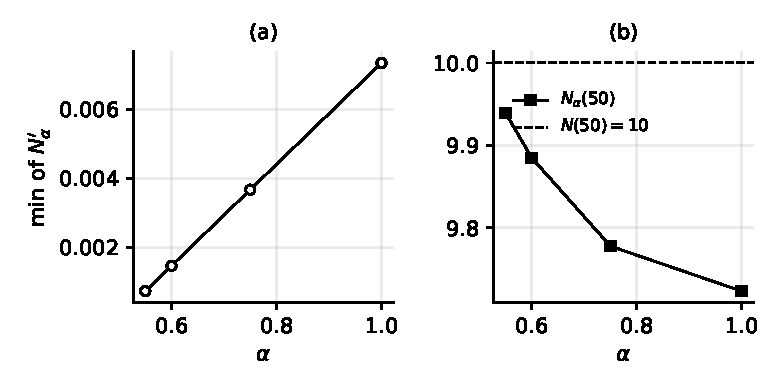
\includegraphics[width=\textwidth]{fig/ht_yor.pdf}
\caption{(a) The minimum over $t$ of the Thorin density $N_\alpha'(t)=\pi^{-1}\Re\,\xi'/\xi(\alpha+it)$ of the base point laws on $[0,50]$, attained at $t=0$, for $\alpha=1,0.75,0.6,0.55$. (b) The values $N_\alpha(50)$ against $N(50)=10$. Only these summary values are stored, so the curves on $[0,50]$ are not drawn (computed).}\label{ht:fig:yor}
\end{figure}

Dirichlet means, the other main theme of \cite{JRY}, need a Thorin measure of finite total mass $\theta$, in which case the GGC is $\gamma_\theta\cdot D_\theta$ with $D_\theta$ a Dirichlet mean \cite[(31) to (35)]{JRY}. % UNCHECKED: equation numbers of JRY not verified
The Thorin measures of $\mu$ and of every $\mu^{(\alpha)}$ with $\alpha\ge\sup_\rho\Re\rho$ have infinite mass. For the truncation $\mu_N=\sum_{n\le N}\varepsilon_n/\gamma_n^2$ the representation holds with $\theta=N$, but $D_N$ tends to $\frac1N\sum_{n\le N}\gamma_n^{-2}\to0$ \cite[Proposition 1.7]{JRY}, % UNCHECKED: proposition number of JRY not verified
so it degenerates in the limit and carries no information about $\mu$.

\subsection{Moments and the Barnes function}
Nikeghbali and Yor \cite{NY09} express the Barnes $G$ function, and through it the Keating and Snaith moments of characteristic polynomials of random unitary matrices, by sums and products of GGC variables (see Section~\ref{ag:sec:moments}). This links GGCs to the conjectured moments of $\zeta$ on the critical line, but moments of $|\zeta(\frac12+it)|$ do not locate zeros, and we see no route from it to the positivity of the Thorin measure of $\mu$.

\subsection{Assessment}
Yor's work supplies three things this programme can use: a Brownian meaning for P\'olya's kernel and hence for the harmonic mean form of $\mu$ (Proposition~\ref{ht:prop:bpy}), exactly solvable models of $\mu$ and of its failure modes in the hyperbolic laws, and a pathwise coupling of the base point laws through the Wiener and Gamma representation (Proposition~\ref{ht:prop:wg}). It does not supply the arithmetic. Proposition~\ref{ht:prop:dhtheta} shows that the positivity and symmetry behind the Biane, Pitman and Yor variable hold for Davenport and Heilbronn too, so they cannot imply RH; the Brownian interpretation of $\theta$ is the one ingredient that might separate the two.

\section{The Davenport Heilbronn test}\label{ht:sec:dh}

Every proposed argument must fail for the Davenport Heilbronn function $f_{DH}$ \cite{DH36}, which has the functional equation $\xi_{DH}(s)=\xi_{DH}(1-s)$ with $\xi_{DH}(s)=(5/\pi)^{s/2}\Gamma(\frac{s+1}2)f_{DH}(s)$, no Euler product, and zeros off the line; the zero at $0.808517182456637+85.6993484853776\,i$ is classical \cite{Spira94} (see Section~\ref{mi:sec:quasi} for the function and its zeros). We confirmed it by the argument principle (one zero in the box $[0.78,0.84]\times[85.67,85.73]$, at two step sizes). Its reciprocal law passes every positivity test we can compute: the Taylor coefficients of $\xi_{DH}(\frac12+\sqrt s)/\xi_{DH}(\frac12)$ have all contiguous Toeplitz minors positive up to order $10$ over the first $100$ indices (computed; the check ran to order $14$ and index $119$ at two precisions, which agree to $80$ digits, not an interval proof), indistinguishable from those of $\xi$, as the angle theorem predicts (Section~\ref{ht:sec:angle}). For hitting times the test rules out the de Bruijn and Newman route and the harmonic mean route unless the Euler product enters them, and it rules out any argument that uses only an archimedean factor of this growth and the functional equation.
